
\chapter{Introduction}\label{C:intro}

\begin{addmargin}[2.5em]{0em}% 1em left, 2em right
\textit {Soon upon waking up in the morning, university student Stephen grabs his mobile phone and checks for incoming e-mails, unread-messages, and social media network updates. He gets ready to head to university. Last minute 	before departing, he uses his mobile application to check his class schedules and confirm the bus schedule. On his way to the bus station, he listens to music on his mobile phone. He also texts his classmates about meeting up for lunch and replies to a discussion board thread about assignments that are due the next day. Using another mobile application, Stephen creates a list of assignments and sets submission notifications for each assignment. After class, he gets together with his classmates and work on a group assignment together. They discuss their response to the assignment topic, and each person record notes on their own laptop. On the way back from university, Stephen 	posts on a closed group chat-room reminding his classmates about the 	assignment's due date. With his study and course work organised for the day, he relaxes and watches live streaming music videos.}
\end{addmargin}
\hfill

\noindent The advance of mobile technology along with the wide-spread popularity of mobile devices have transformed our societies and altered many facets of our lives.  In response to this transformation, more educational institutions are extending their education platforms to encompass mobile-based learning and teaching. This allows students to obtain knowledge regardless of their geographic locations. 

The importance of distance learning is highlighted by its potential to fulfil Goal 2 of the 8 United Nations (UN) Millennium Development Goals. The second UN Millennium Development Goal aims to ensure that by 2015, every child would be able to complete primary school courses. Due to various barriers inhibiting access to education such as locations of available schools, cost of studying, language barrier, and gender inequality, the goal has yet to be achieved. However, mobile devices have the potential to reduce some of these barriers, by assisting students at any level in accessing learning materials, promote distance teaching and learning globally, and ultimately help achieve the said goal outlined by the UN.

Although mobile devices have the potential to promote distance learning and teaching, they are not purposefully designed to be educational tools. Owing to the need to ensure mobility when using these devices, the entailing hardware and software limitations present unique challenges when mobile devices are being used in educational context. Compared to traditional desktop computers or laptops, it is more difficult for mobile devices to deliver large quantities of learning content and provide advanced application functionalities or features to support such content. These limitations serve as a reminder that shifting educational platforms to mobile learning requires deliberate planning and considerations. 

This thesis aims to establish a set of design guidelines grounded in learning principles to drive effective design and evaluation for mobile learning applications, and address some of the limitations of using mobile devices as educational tools for distance learning and teaching.

\section{Problem context}
Mobile learning or m-learning is the process of learning and teaching via mobile devices such as mobile phones, tablets, and Personal Digital Assistants (PDAs). M-learning has remarkable potentials as a mode of education, such as facilitating personalised learning, supporting a cooperative learning environment where many students and their instructors are physically remote from each other, and providing flexibility around learning time and locations for students. 

	Despite these promises, m-learning faces some important challenges due to software and hardware limitations associated with mobile devices (e.g., small screen size, low screen resolution, lack of efficient data entry capability, small storage, slow processing speed, and short battery life). Furthermore, m-learning introduces new complexity pedagogically. It becomes more difficult to track students' learning efficiency and engagement because m-learning enables their learning process to occur without instructors' supervision. Although there are various researches focused on developing m-learning applications, only a few established design guidelines based upon learning principles to address this complexity. 

	Transactional Distance Theory (TDT) is a long-standing theory primarily applied in the field of distance education. According to the theory, students feel disconnected and isolated when they were physical separated from their instructors and other students. It introduced three contributing factors, namely dialogue, course structure, and learner autonomy. 

This thesis applied the principles presented by the theory to form one part of the design guidelines, in order to observe: 

\hfill
\begin{addmargin}[1.5em]{1.5em}
\textit{1. "Can TDT principles be used to construct design guidelines that affect student engagement on m-learning education application?}
\end{addmargin}
\hfill 

While the TDT provides distance learning principles, it does not deal with interface design techniques that are crucial to the success of any application. As a result, the thesis drew upon interface design techniques for m-learning developed from heuristic evaluations created for evaluating general software and e-learning. These techniques formed the other part of the design guidelines from this thesis, from which the following observation is considered: 

\hfill
\begin{addmargin}[1.5em]{1.5em}
\textit{2. "Can interface design techniques be adopted from heuristic evaluation criteria to complement the design guidelines based on TDT principles and improve student engagement?"}
\end{addmargin}
\hfill 

	In addition to ensuring the quality of the m-learning application, identifying and understanding target users is also critical to the success of the design, particularly at the early stage of the application development process. It facilitates the selection of appropriate and meaningful learning content that can be delivered on mobile technology with limited resources, while highlighting the necessary adjustments required to match students' preferences and abilities. Lastly, TDT also emphasises the importance of "Learner Autonomy" on students' learning effectiveness. At the initial stage of the m-learning application development process, two user studies were carried out to create user personas and inform the m-learning application design. At the application's evaluation stage, the thesis observed: 

\hfill
\begin{addmargin}[1.5em]{1.5em}
\textit{3. "Is there any correlation between the engagement level and learner autonomy?"}
\end{addmargin}

\section{Methodology}
The m-learning application design guidelines are developed based on outputs from three phases. In order to validate the completeness and efficiency of the developed guidelines, all three phases were repeated once in cycle. Figure 1.1 illustrates the research process. 

\begin{figure}[!hbt]
\centering
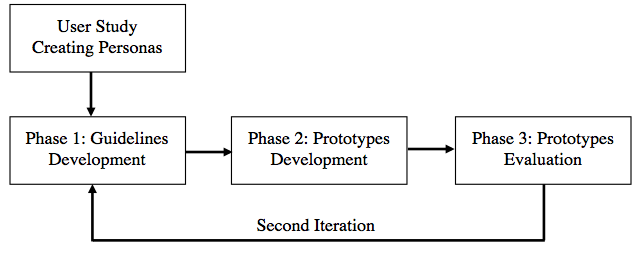
\includegraphics[width=1.0 \textwidth]{chapter1}
\caption{Research process cycle}
\end{figure}

\textbf{Guidelines Development}- the first phase focused on establishing the design guidelines. In the first iteration, we developed theoretical guidelines based on the principles of TDT. The theory was published in general distance education context. The thesis examined how the theory could be adjusted to guide the design of modern m-learning education context. The thesis also reviewed some past literature to validate the appropriateness and accuracy of the adjustment. 

Concurrently, a \textbf{User Study} was launched in an effort to understand our target m-learning application users and provide an indication towards the practicality, possibility, and appropriateness of such theoretical-based design guidelines. This study was carried out through an online survey targeted at first year computer science and engineering students at Victoria University of Wellington, New Zealand. 

In the second iteration of the guidelines development process, the interface design techniques (i.e., heuristic evaluation) were incorporated into the theoretical design guidelines we developed in the first iteration. 

\textbf{Prototypes Development} - the second phase focused on designing m-learning application prototypes following the design guidelines for and user study findings we harnessed in the first phase. 

In order to compare if the guidelines based on TDT could engage students during their learning process, two prototypes were designed. One prototype followed the TDT guidelines and provided learning support mechanisms as suggested by TDT, whereas the other prototype did not provide any of such mechanism. Both prototypes used the same interface design and presented the same learning content, with the purpose of eliminating usability as a variable that could influence the comparison process. 

\textbf{Prototypes Evaluation}- the last phase focused on evaluating the prototypes. A post-questionnaire was used to measure students' engagement. The questionnaire was developed based on many credible literatures that offered student engagement measuring scale. It was a quantitative measurement of students' self-evaluation on how they engaged with the prototypes. Additionally, video recordings of students interacting with the prototypes were captured as part of interface design evaluation, and formed the qualitative findings of this thesis. An online analytics tool (i.e., Google Analytics for mobile devices) was used to track and report on the performance statistically as a backup evaluation tool. 

The quantitative results and qualitative findings from each prototype were compared and analysed. These results helped determine if the prototype following the design guidelines could engage students better than the other prototype where such implementation was absent. Furthermore, the results act as an assessment mechanism to determine if the interface design was appropriate. In this phase, students' learning autonomy was also measured using self-evaluation with paper-based questionnaire and observation of the participants' tasks performance in order to gage any potential between learning autonomy and student engagement. 

\section{Contributions}
This thesis makes three contributions to m-learning: 

\begin{enumerate}

\item Draws on TDT to contribute new design knowledge with emphasis on the concept of dialogue, course structure, and learner autonomy, which can be incorporated into the design and evaluation process of m-learning applications. 

\item Develops new proof-of-concept prototypes design guidelines for m-learning application based on learning principles and empirical studies to ensure learning engagement. 

\item Presents a critique towards appropriateness, ability, and possibility of TDT in guiding the design of modern education platform such as m-learning. 

\end{enumerate}

\section{Delimitation and Limitations}

To evaluate the guidelines, an m-learning application was designed a specific smart phone. Its specifications limited participants' performance, defined scope for the interface design and design suggestions proposed. 

A reward strategy (i.e., grocery voucher) was employed to recruit student participants, encourage them to be motivated and be willing to interact with the m-learning application in ways that would be comparable to a real-life application user. This strategy may have influence on the outcome from the "learner autonomy" evaluation. Results collected from the Prototype Evaluation phase indicated the absence of any participant with low autonomy level. 

Learning content presented in the application are based on curriculum for undergraduate degree programs within the field of Computer Science and Computing-based Engineering. These subjects were chosen based on researcher and supervisors' field of expertise. There was no prior assessment of participants' level of knowledge and understanding of these subjects, which might have an effect on their level of attention and engagement to learning the subjects via the application. 

In the first evaluation iteration, an erroneous function within the application required participants to reset the application in order to continue with their learning process. The potential effect of this defect on participants' engagement with the first iteration application prototype have been documented in the relevant analysis and results sections. This defect was resolved in the second iteration prototypes. 

\section{Thesis Structure Outline}

\textbf{Chapter 2 - Background and Related Work} defined relevant terms including m-learning, TDT which the m-learning guidelines developed within this thesis is based upon, user persona which represented target learners, heuristic evaluations which complement the theoretical design guidelines, and student engagement which is the key evaluation of m-learning applications, explored existing m-learning design guidelines and its applications, exiting m-learning application development and evaluation studies, and existing studies towards teaching and learning that consisted of TDT concepts, introduces some past literatures that contributed in this thesis including persona development process, heuristic evaluation techniques, and student engagement's evaluation scale. 

\textbf{Chapter 3 - First Theoretical Design Guidelines and User Study} presents how the original concept of TDT proposed in general distance education context is translated to modern education context of m-learning application in this thesis. It also presents a primary user study aimed to understand the target m-learning application users and describe their experience and willingness towards using such applications. A final user persona is selected based on the primary user study, to be used subsequent phases of the thesis. 

\textbf{Chapter 4 - First Prototype Development} presents two application prototype designs based on the theoretical design guidelines and the final user persona created in chapter 3. It demonstrates the quantitative results gathered on the level of students' engagement with their learning process through using the prototypes, and qualitative findings on the prototypes' interface design based on their interaction with the prototype applications. The results and findings are analysed and used to critique the first iteration theoretical design guidelines, and provide suggestions on potential improvements to be incorporated in the second iteration. 

\textbf{Chapter 5 - Second Design Guidelines} presents development process of heuristics evaluation guidelines for m-learning application based on the past literature about presented in chapter 2, explores how the invented heuristic evaluation guidelines were used by experts to evaluate the first prototype developed in chapter 4, explains incorporation of the heuristic evaluation guidelines into the existing theoretical design guidelines we proposed in chapter 3. 

\textbf{Chapter 6 - Second Prototype Development} presents two new application prototypes designed using the improved theoretical design guidelines, new interface design developed based on heuristic evaluation techniques, and the user persona created in chapter 3. Similar to the first iteration, this chapter shows the new quantitative results on students' engagement level and new qualitative findings on the prototypes' interface design using the new prototypes. The results and findings are then analysed and used to critique the final theoretical design guidelines and demonstrate how the interface design improvement affects engagement quantitatively and learning efficiency qualitatively. 

\textbf{Chapter 7 - Conclusion} summarises the thesis and describes its three major contributions to the field of m-learning. By placing these contributions into the context of related works discussed in chapter 2, this chapter further presents considerations and possible future approaches for m-learning application design guidelines. 

\section{Publications}

Some of the work presented in the thesis had been published elsewhere prior to thesis write-up. These publications are the primary works of the author of this thesis, with the co-author providing some supervisions and advice. 

\textbf{Chapter 1} - research motivations, problem context, goals, methodology, and expected contributions were briefly described in \textit{"Mobile Learning Application for Computer Science Students: A Transactional Distance Perspective"}, published in the Proceedings of the 2016 ACM Conference on International Computing Education Research \cite{limtrairut2016mobile}. 

\textbf{Chapter 3} - primary user study, user persona, and initial prototype design were discussed in \textit{"Know the Mobile Learning Application Users - Transactional Distance Perspective"}, published in the Proceedings of the \nth{8} International Conference on Computer Supported Education \cite{limtrairut2016know}. 






























